\documentclass{article}

\usepackage{enumerate}
\usepackage{pdfpages}
\usepackage{mathtools}
\usepackage{listings,multicol}
\usepackage{listings}
\usepackage{amsmath}

\newcommand{\vecn}[1]{\boldsymbol{#1}}
\begin{document}
The basis functions space = $V_j = \left[\phi_{j-1/2},\phi_{j-1/6},\phi_{j+1/6},\phi_{j+1/2}\right]$ over a cell and then $V = \cup_j V_j$
\begin{figure}
\centering
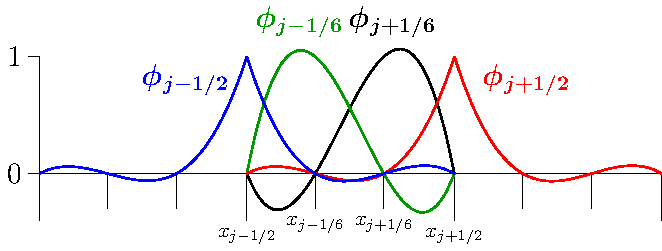
\includegraphics{P3.pdf}
\caption{Basis functions}
\end{figure}

Want to approximate 
\begin{equation}
G = uh
\end{equation}

This becomes in weak form where

\begin{equation}
\int_\Omega G v dx = \int_\Omega uh v dx
\end{equation}

We reduce to finding solutions to 

\begin{equation}
\int_\Omega v dx = \int_\Omega uh v dx
\end{equation}

where $v \in V$. Using the partitioning of domain into cells we have

\begin{equation}
 \sum_j \int_{x_{j-1/2}}^{x_{j+1/2}} G v dx = \sum_j \int_{x_{j-1/2}}^{x_{j+1/2}} uh v dx
\end{equation}

Can write $G$, $u$ and $h$ on basis functions

$$q = \sum_j \left(q_{j-1/2}\phi_{j-1/2} + q_{j-1/6}\phi_{j-1/6} + q_{j+1/6}\phi_{j+1/6}  +q_{j+1/2}\phi_{j+1/2}\right)$$

$$q = \vecn{q} \cdot \vecn{\phi}$$

where $\vecn{q}$ is the vector of all the nodal values and $\vecn{\phi}$ is the vector of all basis functions. 

\begin{equation}
\int_{x_{j-1/2}}^{x_{j+1/2}} G v dx = \int_{x_{j-1/2}}^{x_{j+1/2}} \left(G_{j-1/2}\phi_{j-1/2} + G_{j-1/6}\phi_{j-1/6} + G_{j+1/6}\phi_{j+1/6}  + G_{j+1/2}\phi_{j+1/2}\right) \begin{bmatrix}
\phi_{j-1/2} \\ \phi_{j-1/6}\\ \phi_{j+1/6} \\\phi_{j+1/2}
\end{bmatrix} 
\end{equation}


\begin{equation}
= \int_{x_{j-1/2}}^{x_{j+1/2}} \begin{bmatrix}
G_{j-1/2}\phi_{j-1/2}\phi_{j-1/2} + G_{j-1/6}\phi_{j-1/6}\phi_{j-1/2} + G_{j+1/6}\phi_{j+1/6}\phi_{j-1/2}  + G_{j+1/2}\phi_{j+1/2}\phi_{j-1/2} \\
G_{j-1/2}\phi_{j-1/2}\phi_{j-1/6} + G_{j-1/6}\phi_{j-1/6}\phi_{j-1/6} + G_{j+1/6}\phi_{j+1/6}\phi_{j-1/6}  + G_{j+1/2}\phi_{j+1/2}\phi_{j-1/6} \\
G_{j-1/2}\phi_{j-1/2}\phi_{j+1/6} + G_{j-1/6}\phi_{j-1/6}\phi_{j+1/6} + G_{j+1/6}\phi_{j+1/6}\phi_{j+1/6}  + G_{j+1/2}\phi_{j+1/2}\phi_{j+1/6} \\
G_{j-1/2}\phi_{j-1/2}\phi_{j+1/2} + G_{j-1/6}\phi_{j-1/6}\phi_{j+1/2} + G_{j+1/6}\phi_{j+1/6}\phi_{j+1/2}  + G_{j+1/2}\phi_{j+1/2}\phi_{j+1/2} 
\end{bmatrix}
\end{equation}

\begin{equation}
= \int_{x_{j-1/2}}^{x_{j+1/2}} \begin{bmatrix}
\phi_{j-1/2}\phi_{j-1/2} & \phi_{j-1/6}\phi_{j-1/2} & \phi_{j+1/6}\phi_{j-1/2}  & \phi_{j+1/2}\phi_{j-1/2} \\
\phi_{j-1/2}\phi_{j-1/6} & \phi_{j-1/6}\phi_{j-1/6} & \phi_{j+1/6}\phi_{j-1/6} & \phi_{j+1/2}\phi_{j-1/6} \\
\phi_{j-1/2}\phi_{j+1/6} & \phi_{j-1/6}\phi_{j+1/6} & \phi_{j+1/6}\phi_{j+1/6}  & \phi_{j+1/2}\phi_{j+1/6} \\
\phi_{j-1/2}\phi_{j+1/2} & \phi_{j-1/6}\phi_{j+1/2} & \phi_{j+1/6}\phi_{j+1/2}  & \phi_{j+1/2}\phi_{j+1/2} 
\end{bmatrix} \begin{bmatrix}
G_{j-1/2} \\ G_{j-1/6} \\ G_{j+1/6}   \\ G_{j+1/2}
\end{bmatrix} 
\end{equation}

\begin{multline}
=  \begin{bmatrix}
\int_{x_{j-1/2}}^{x_{j+1/2}}  \phi_{j-1/2}\phi_{j-1/2}  dx &  \int_{x_{j-1/2}}^{x_{j+1/2}} \phi_{j-1/6}\phi_{j-1/2}  dx&  \int_{x_{j-1/2}}^{x_{j+1/2}} \phi_{j+1/6}\phi_{j-1/2}  dx & \int_{x_{j-1/2}}^{x_{j+1/2}} \phi_{j+1/2}\phi_{j-1/2} dx \\
\int_{x_{j-1/2}}^{x_{j+1/2}}  \phi_{j-1/2}\phi_{j-1/6}  dx &  \int_{x_{j-1/2}}^{x_{j+1/2}} \phi_{j-1/6}\phi_{j-1/6}  dx&  \int_{x_{j-1/2}}^{x_{j+1/2}} \phi_{j+1/6}\phi_{j-1/6}  dx & \int_{x_{j-1/2}}^{x_{j+1/2}} \phi_{j+1/2}\phi_{j-1/6} dx \\
\int_{x_{j-1/2}}^{x_{j+1/2}}  \phi_{j-1/2}\phi_{j+1/6}  dx &  \int_{x_{j-1/2}}^{x_{j+1/2}} \phi_{j-1/6}\phi_{j+1/6}  dx&  \int_{x_{j-1/2}}^{x_{j+1/2}} \phi_{j+1/6}\phi_{j+1/6}  dx & \int_{x_{j-1/2}}^{x_{j+1/2}} \phi_{j+1/2}\phi_{j+1/6} dx \\
\int_{x_{j-1/2}}^{x_{j+1/2}}  \phi_{j-1/2}\phi_{j+1/2}  dx &  \int_{x_{j-1/2}}^{x_{j+1/2}} \phi_{j-1/6}\phi_{j+1/2}  dx&  \int_{x_{j-1/2}}^{x_{j+1/2}} \phi_{j+1/6}\phi_{j+1/2}  dx & \int_{x_{j-1/2}}^{x_{j+1/2}} \phi_{j+1/2}\phi_{j+1/2} dx \\
\end{bmatrix} \\ \begin{bmatrix}
G_{j-1/2} \\ G_{j-1/6} \\ G_{j+1/6}   \\ G_{j+1/2}
\end{bmatrix} 
\end{multline}


for the $uh$ term
\begin{multline}
\int_{x_{j-1/2}}^{x_{j+1/2}} uhv dx = \\
 \int_{x_{j-1/2}}^{x_{j+1/2}} \left(u_{j-1/2}\phi_{j-1/2} + u_{j-1/6}\phi_{j-1/6} + u_{j+1/6}\phi_{j+1/6}  + u_{j+1/2}\phi_{j+1/2}\right) \\
  \left(h_{j-1/2}\phi_{j-1/2} + h_{j-1/6}\phi_{j-1/6} + h_{j+1/6}\phi_{j+1/6}  + h_{j+1/2}\phi_{j+1/2}\right) \\ \begin{bmatrix}
\phi_{j-1/2} \\ \phi_{j-1/6}\\ \phi_{j+1/6} \\\phi_{j+1/2}
\end{bmatrix} 
\end{multline}


\begin{multline}
\int_{x_{j-1/2}}^{x_{j+1/2}} uhv dx = \\
\int_{x_{j-1/2}}^{x_{j+1/2}} \left(\vecn{u}_j \cdot \vecn{\phi}_j\right) \left(\vecn{h}_j \cdot \vecn{\phi}_j\right)  \begin{bmatrix}
\phi_{j-1/2} \\ \phi_{j-1/6}\\ \phi_{j+1/6} \\\phi_{j+1/2}
\end{bmatrix} 
\end{multline}

\begin{equation}
\int_{x_{j-1/2}}^{x_{j+1/2}} uhv dx = \\
\int_{x_{j-1/2}}^{x_{j+1/2}} \left(\vecn{u}_j \cdot \vecn{\phi}_j\right) \vecn{\phi}_j \left(\vecn{h}_j \cdot \vecn{\phi}_j\right)  
\end{equation}

\begin{equation}
\int_{x_{j-1/2}}^{x_{j+1/2}} uhv dx = \\
\int_{x_{j-1/2}}^{x_{j+1/2}} \left(\vecn{u}_j^T \vecn{\phi}_j\right) \vecn{\phi}_j \left(\vecn{h}_j^T \vecn{\phi}_j\right)  
\end{equation}
\begin{equation}
\int_{x_{j-1/2}}^{x_{j+1/2}} uhv dx = \\
\int_{x_{j-1/2}}^{x_{j+1/2}} \left(\vecn{h}_j^T \vecn{\phi}_j\right)  \vecn{\phi}_j  \left(\vecn{\phi}_j^T \vecn{u}_j\right) 
\end{equation}
\begin{equation}
\int_{x_{j-1/2}}^{x_{j+1/2}} uhv dx = \\
\int_{x_{j-1/2}}^{x_{j+1/2}} \left(\vecn{h}_j^T \vecn{\phi}_j\right)  \left(\vecn{\phi}_j  \vecn{\phi}_j^T \right) \vecn{u}_j
\end{equation}
\begin{equation}
\int_{x_{j-1/2}}^{x_{j+1/2}} uhv dx = \\
\int_{x_{j-1/2}}^{x_{j+1/2}} \left(\vecn{h}_j^T \vecn{\phi}_j\right)  \left(\vecn{\phi}_j  \vecn{\phi}_j^T \right) \vecn{u}_j
\end{equation}

\begin{equation}
\int_{x_{j-1/2}}^{x_{j+1/2}} uhv dx = \\
\int_{x_{j-1/2}}^{x_{j+1/2}} \left(\vecn{h}_j^T \vecn{\phi}^2_j \vecn{\phi}_j^T \right) \vecn{u}_j
\end{equation}






\end{document}